\documentclass[]{book}
\usepackage{lmodern}
\usepackage{amssymb,amsmath}
\usepackage{ifxetex,ifluatex}
\usepackage{fixltx2e} % provides \textsubscript
\ifnum 0\ifxetex 1\fi\ifluatex 1\fi=0 % if pdftex
  \usepackage[T1]{fontenc}
  \usepackage[utf8]{inputenc}
\else % if luatex or xelatex
  \ifxetex
    \usepackage{mathspec}
  \else
    \usepackage{fontspec}
  \fi
  \defaultfontfeatures{Ligatures=TeX,Scale=MatchLowercase}
\fi
% use upquote if available, for straight quotes in verbatim environments
\IfFileExists{upquote.sty}{\usepackage{upquote}}{}
% use microtype if available
\IfFileExists{microtype.sty}{%
\usepackage{microtype}
\UseMicrotypeSet[protrusion]{basicmath} % disable protrusion for tt fonts
}{}
\usepackage{hyperref}
\hypersetup{unicode=true,
            pdftitle={Bayesian Modeling},
            pdfauthor={Jim Albert and Jingchen Hu},
            pdfborder={0 0 0},
            breaklinks=true}
\urlstyle{same}  % don't use monospace font for urls
\usepackage{natbib}
\bibliographystyle{apalike}
\usepackage{longtable,booktabs}
\usepackage{graphicx,grffile}
\makeatletter
\def\maxwidth{\ifdim\Gin@nat@width>\linewidth\linewidth\else\Gin@nat@width\fi}
\def\maxheight{\ifdim\Gin@nat@height>\textheight\textheight\else\Gin@nat@height\fi}
\makeatother
% Scale images if necessary, so that they will not overflow the page
% margins by default, and it is still possible to overwrite the defaults
% using explicit options in \includegraphics[width, height, ...]{}
\setkeys{Gin}{width=\maxwidth,height=\maxheight,keepaspectratio}
\IfFileExists{parskip.sty}{%
\usepackage{parskip}
}{% else
\setlength{\parindent}{0pt}
\setlength{\parskip}{6pt plus 2pt minus 1pt}
}
\setlength{\emergencystretch}{3em}  % prevent overfull lines
\providecommand{\tightlist}{%
  \setlength{\itemsep}{0pt}\setlength{\parskip}{0pt}}
\setcounter{secnumdepth}{5}
% Redefines (sub)paragraphs to behave more like sections
\ifx\paragraph\undefined\else
\let\oldparagraph\paragraph
\renewcommand{\paragraph}[1]{\oldparagraph{#1}\mbox{}}
\fi
\ifx\subparagraph\undefined\else
\let\oldsubparagraph\subparagraph
\renewcommand{\subparagraph}[1]{\oldsubparagraph{#1}\mbox{}}
\fi

%%% Use protect on footnotes to avoid problems with footnotes in titles
\let\rmarkdownfootnote\footnote%
\def\footnote{\protect\rmarkdownfootnote}

%%% Change title format to be more compact
\usepackage{titling}

% Create subtitle command for use in maketitle
\providecommand{\subtitle}[1]{
  \posttitle{
    \begin{center}\large#1\end{center}
    }
}

\setlength{\droptitle}{-2em}

  \title{Bayesian Modeling}
    \pretitle{\vspace{\droptitle}\centering\huge}
  \posttitle{\par}
    \author{Jim Albert and Jingchen Hu}
    \preauthor{\centering\large\emph}
  \postauthor{\par}
      \predate{\centering\large\emph}
  \postdate{\par}
    \date{2019-08-05}

\usepackage{booktabs}
\usepackage{amsthm}
\makeatletter
\def\thm@space@setup{%
  \thm@preskip=8pt plus 2pt minus 4pt
  \thm@postskip=\thm@preskip
}
\makeatother

\begin{document}
\maketitle

{
\setcounter{tocdepth}{1}
\tableofcontents
}
\hypertarget{preface}{%
\chapter{Preface}\label{preface}}

\hypertarget{intro}{%
\chapter{Learning About a Binomial Probability}\label{intro}}

\hypertarget{introduction-thinking-about-a-proportion-subjectively}{%
\section{Introduction: Thinking About a Proportion Subjectively}\label{introduction-thinking-about-a-proportion-subjectively}}

In previous chapters, we have seen many examples involving drawing color balls from a box. In those examples, we are given the numbers of balls of various colors in the box, and we consider questions related to calculating probabilities. For example, there are 40 white and 20 red balls in a box. If you draw two balls at random, what is the probability that both balls are white?

Here we consider a new scenario where we do not know the proportions of color balls in the box. That is, in the previous example, we only know that there are two kinds of color balls in the box, but we don't know 40 out of 60 of the balls are white (proportion of white = \(2/3\)) and 20 out of the 60 of the balls are red (proportion of red = \(1/3\)). How can we learn about the proportions of white and red balls? Since counting 60 balls can be tedious, how can we infer those proportions by drawing a sample\index{sample} of balls out of the box and observe the colors of balls in the sample\index{sample}? This becomes an inference\index{inference} question, because we are trying to infer the proportion\index{proportion} \(p\) of the population\index{population}, based on a sample\index{sample} from the population\index{population}.

Let's continue discussing the scenario where we are told that there are 60 balls in total in a box, and the balls are either white or red. We do not know the count of balls of each of the two colors.
We are given the opportunity to take a random sample\index{random!random sample} of 10 balls out of these 60 balls. We are interested in the quantity \(p\), the proportion\index{proportion} of red balls in the 60 balls. How can we infer \(p\), the proportion\index{proportion} of red balls in the population\index{population} (i.e.~the 60 balls), based on the numbers of red and white balls we observe in the sample\index{sample} (i.e.~the 10 balls)?

Proportions are like probabilities. Recall in Chapter 1 three views of a probability were discussed. We briefly review them here, and state the specific requirements to obtain each view.

\begin{enumerate}
\def\labelenumi{\arabic{enumi}.}
\item
  The classical view: one needs to write down the sample space\index{sample!sample space} where each outcome is equally likely.
\item
  The frequency view: one needs to repeat the random experiments\index{random!random experiment} many times under identical conditions.
\item
  The subjective view: one needs to express one's opinion about the likelihood\index{likelihood} of a one-time event.
\end{enumerate}

The classical view does not seem to work here, because we only know there are two kinds of color balls and the total number of balls is 60. Even if we take a sample\index{sample} of 10 balls, we are only going to observe the proportion\index{population} of red balls in the sample\index{sample}. There does not seem to be a way for us to write down the sample space\index{sample!sample space} where each outcome is equally likely.

The frequency view would work here. One could treat the process of obtaining a sample\index{sample} (i.e.~taking a random sample\index{random!random sample} of 10 balls from the box) as an experiment\index{experiment}, and obtain a sample proportion\index{sample!sample proportion} \(\hat{p}\) from the experiment\index{experiment}. One then could repeat the experiment\index{experiment} many times under the same condition, get many sample proportions\index{sample!sample proportion} \(\hat{p}\), and summarize all the \(\hat{p}\). When one repeats the experiment\index{experiment} enough times (a large number), one gets a good sense about the proportion \(p\) of red balls in the population\index{population} of 60 balls in the box. This process is doable, but tedious, time-consuming, and prone to errors.

The subjective view perceives the unknown proportion \(p\) subjectively. It does require one to express his or her opinion about the value of \(p\), and he or she could be skeptical and unconfident about the opinion. In Chapter 1, a calibration experiment\index{experiment} was introduced to help one sharpen an opinion about the likelihood\index{likelihood} of an event by comparisons with opinion about the likelihood\index{likelihood} of other events. In this chapter and the chapters to follow, we introduce the key ideas and practice about thinking subjectively about unknowns and quantify one's opinions about the values of these unknowns using probability distributions\index{probability!probability distribution}.

As an example, let's think about plausible values for the proportion \(p\) of red balls. As \(p\) is a proportion\index{proportion}, it can take any possible value between 0 and 1. In the calibration experiment\index{experiment} introduced in Chapter 1, we focus on the scenario where only one value of \(p\) is of interest. For example, when one thinks that \(p\) is 0.5, it is saying that one's opinion about the probability of the value \(p=0.5\) is one. When we phrase it this way (``one's opinion about the probability of \(p=0.5\) is one"), it sounds like a very strong opinion, because one only allows \(p\) to take one possible value, and gives probability one of that happening. Since one typically has no thought about the exact value of the proportion\index{proportion} \(p\), setting one possible value for the proportion with probability one seems too strong.

Instead suppose that the proportion\index{proportion} \(p\) can take multiple values between 0 and 1. In particular, let's consider two scenarios, in both \(p\) can take 10 different values, denoted by set \(A\).

\begin{eqnarray}
A = \{0.1, 0.2, 0.3, 0.4, 0.5, 0.6, 0.7, 0.8, 0.9, 1.0\}
\end{eqnarray}

Though \(p\) can take the same 10 multiple values in both scenarios, we assign different probabilities to each possible value.

\begin{enumerate}
\item[-] Scenario 1: 
\begin{eqnarray}
f_1(A) = (0.1, 0.1, 0.1, 0.1, 0.1, 0.1, 0.1, 0.1, 0.1, 0.1)
\end{eqnarray}
\item[-] Scenario 2: 
\begin{eqnarray}
f_2(A) = (0.05, 0.05, 0.05, 0.175, 0.175, 0.175, 0.175, 0.05, 0.05, 0.05) \nonumber \\
\end{eqnarray}
\end{enumerate}

To visually compare the values of two probability distributions\index{probability!probability distribution} \(f_1(A)\) and \(f_2(A)\), we plot \(f_1(A)\) and \(f_2(A)\) on the same graph as in Figure \ref{fig:RedBallProp_prob}.

\begin{figure}[htb]
\begin{center}
\includegraphics[scale=0.4]{figures/chapter6/RedBallProp_prob.pdf}
\caption{\label{fig:RedBallProp_prob} The same ten possible values of $p$, but two sets of probabilities.}
\end{center}
\end{figure}

Figure \ref{fig:RedBallProp_prob} labels the \(x\)-axis as the values of \(p\) (range from 0 to 1), \(y\)-axis as the probabilities (range from 0 to 1). For both panels, there are ten bars, each representing the possible values of \(p\) in the set \(A = \{0.1, 0.2, 0.3, 0.4, 0.5, 0.6, 0.7, 0.8, 0.9, 1.0\}\).

The probability assignment in \(f_1(A)\) is called a discrete\index{discrete} Uniform distribution\index{Uniform!Uniform distribution}, where each possible value of the proportion\index{proportion} \(p\) is equally likely. Since there are ten possible values of \(p\), each value gets assigned a probability of \(1/10 = 0.1\). This assignment expresses the opinion that \(p\) can be any value from the set \(A = \{0.1, 0.2, 0.3, 0.4, 0.5, 0.6, 0.7, 0.8, 0.9, 1.0\}\), and each value has a probability of \(0.1\).

The probability assignment in \(f_2(A)\) is also discrete\index{discrete}, however, we do not see a Uniform distribution\index{Uniform!Uniform distribution} pattern of the probabilities across the board. What we see is that the probabilities of the first three values (0.1, 0.2, and 0.3) and last three (0.8, 0.9, and 1.0) values of \(p\) are each \(1/3.5\) of that of the middle four (0.4, 0.5, 0.6, and 0.7) values. The shape of the bins reflects the opinion that the middle values of \(p\) are 3.5 times as likely as the extreme values of \(p\).

Both sets of probabilities follow the three probability axioms\index{probability!probability axiom} in Chapter 1. One sees that within each set,

\begin{enumerate}
\def\labelenumi{\arabic{enumi}.}
\item
  Each probability is nonnegative;
\item
  The sum of the probabilities is 1;
\item
  The probability of mutually exclusive\index{mutually exclusive} values is the sum of probability of each value, e.g.~probability of \(p = 0.1\) or \(p = 0.2\) is \(0.1 + 0.1\) in \(f_1(A)\), and \(0.05 + 0.05\) in \(f_2(A)\).
\end{enumerate}

In this introduction, we have presented a way to think about proportions subjectively. We have introduced a way to allow multiple values of \(p\), and perform probability assignments that follow the three probability axioms\index{probability!probability axiom}. One probability distribution\index{probability!probability distribution} expresses a unique opinion about the proportion\index{proportion} \(p\).

To answer our inference\index{inference} question ``what is the proportion\index{proportion} of red balls in the box'', we will take a random sample\index{random!random sample} of 10 balls, and use the observed proportion\index{proportion} of red balls in that sample\index{sample} to sharpen and update our belief about \(p\). Bayesian inference\index{Bayesian!Bayesian inference} is a formal method for implementing this way of thinking and problem solving, including three general steps.

\begin{itemize}
\item
  Step 1: \{(\bf Prior)\index{prior}\}: express an opinion about the location\index{location} of the proportion\index{proportion} \(p\) before sampling\index{sampling}.
\item
  Step 2: \{(\bf Data/Likelihood)\index{likelihood}\}: take the sample\index{sample} and record the observed proportion\index{proportion} of red balls.
\item
  Step 3: \{(\bf Posterior)\index{posterior}\}:use Bayes' rule\index{Bayes' rule} to sharpen and update the previous opinion about \(p\) given the information from the sample\index{sample}.
\end{itemize}

As indicated in the parentheses, the first step ``Prior'' constructs \{\it prior\} opinion\index{prior!prior opinion} about the quantity of interest\index{quantity of interest}, and a probability distribution\index{probability!probability distribution} is used (like \(f_1(A)\) and \(f_2(A)\) earlier) to quantify the prior opinion\index{prior!prior opinion}. The name ``prior"\index{prior} indicates that the opinion should be formed before collecting any data.

The second step ``Data" is the process of data collection, where the quantity of interest\index{quantity of interest} is observed in the collected data. For example, if our 10-ball sample\index{sample} contains 4 red balls and 6 white balls, the observed proportion\index{proportion} of red balls is \(4/10 = 0.4\). Informally, how does this information help us sharpen one's opinion about \(p\)? Intuitively one would give more probability to \(p = 0.4\), but it is unclear how the probabilities would be redistributed among the 10 values in \(A\). Since the sum of all probabilities is 1, is it possible that some of the larger proportion\index{proportion} values, such as \(p = 0.9\) and \(p = 1.0\), will receive probabilities of zero? To address these questions, the third step is needed.

The third step ``Posterior'' combines one's prior opinion\index{prior!prior opinion} and the collected data to update one's opinion about the quantity of interest\index{quantity of interest}. Just like the example of observing 4 red balls in the 10-ball sample\index{sample}, one needs a structured way of updating the opinion from prior\index{prior} to posterior\index{posterior}.

Throughout this chapter, the entire inference\index{inference} process will be described for learning about a proportion\index{proportion} \(p\). This chapter will discuss how to express prior opinion\index{prior!prior opinion} that matches with one's belief, how to extract information from the data/likelihood\index{likelihood}, and how to update our opinion to its posterior\index{posterior}, combining our prior\index{prior} and information from the data/likelihood\index{likelihood} in a principled way.

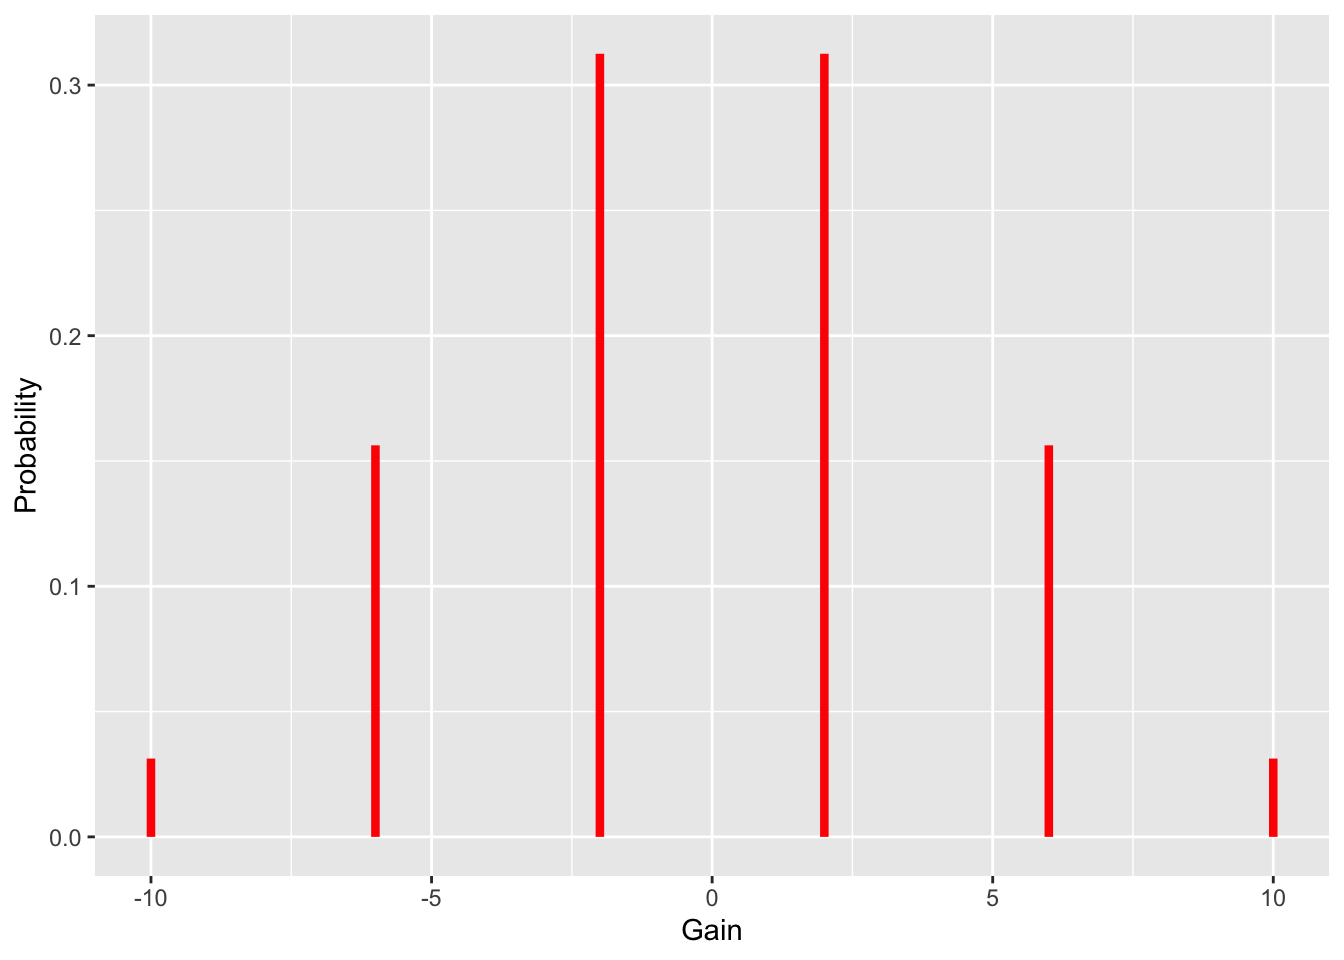
\includegraphics{bookdown-demo_files/figure-latex/unnamed-chunk-1-1.pdf}

\hypertarget{literature}{%
\chapter{Literature}\label{literature}}

Here is a review of existing methods.

\hypertarget{methods}{%
\chapter{Methods}\label{methods}}

We describe our methods in this chapter.

\hypertarget{applications}{%
\chapter{Applications}\label{applications}}

Some \emph{significant} applications are demonstrated in this chapter.

\hypertarget{example-one}{%
\section{Example one}\label{example-one}}

\hypertarget{example-two}{%
\section{Example two}\label{example-two}}

\hypertarget{final-words}{%
\chapter{Final Words}\label{final-words}}

We have finished a nice book.

\bibliography{book.bib,packages.bib}


\end{document}
